\documentclass[11pt,a4paper,twocolumn]{article}
%\usepackage[utf8]{inputenc}
\usepackage[T1]{fontenc}
\usepackage[english]{babel}
\usepackage{amsmath}
\usepackage{amsfonts}
\usepackage{amssymb}
\usepackage{graphicx}
\usepackage{parskip}
\usepackage{lmodern}
\usepackage{braket}
\usepackage{mathtools}
\usepackage[left=2cm,right=2cm,top=2cm,bottom=2cm,bindingoffset=0.5cm]{geometry}
\usepackage{caption}
\usepackage{subcaption}
\usepackage{float}
\usepackage{bm}
\usepackage{booktabs}
\usepackage{scrextend}
\usepackage[font={small,it}]{caption}

\usepackage{color}
\usepackage{fancyvrb}
\usepackage{listings}
\usepackage{bm}
\usepackage[hidelinks]{hyperref}

%%% ALL OF THIS STUFF IS JUST FOR THE CODE
\definecolor{codegreen}{rgb}{0,0.6,0}
\definecolor{codegray}{rgb}{0.5,0.5,0.5}
\definecolor{codepurple}{rgb}{0.58,0,0.82}
\definecolor{backcolour}{rgb}{1,1,1}

\lstdefinestyle{mystyle}{
    backgroundcolor=\color{backcolour},   
    commentstyle=\color{codegreen},
    keywordstyle=\color{magenta},
    numberstyle=\tiny\color{codegray},
    stringstyle=\color{codepurple},
    basicstyle=\ttfamily\footnotesize,
    breakatwhitespace=false,         
    breaklines=true,                 
    captionpos=b,                    
    keepspaces=true,                 
    numbersep=5pt,                  
    showspaces=false,                
    showstringspaces=false,
    showtabs=false,                  
    tabsize=2,
    numbers=left,
    columns=fullflexible
    }
 
\lstset{style=mystyle}
%%% ALL OF THIS STUFF WAS JUST FOR THE CODE


\author{Giovanni Mizzi \\ID 1450441}
\title{\textbf{Complexity in the electoral competition game}}

\begin{document}

\maketitle

\section*{Introduction}
\vspace*{-0.2cm}
Electoral competitions have always been fascinating for Social Scientist. They represent the best way to take decisions the part of humanity who decided to govern itself with democracy could come up, and could be dated back to the ancient Greece. Since the outcome of an electoral competition is something that influences, on different levels, every part of the society, great effort has been put in trying to solve the problem of its prediction.
The traditional model used in Game Theory for this problem is the Hotelling's Game. This is a completely rational model and, starting from some simple assumptions, in a very simple way, it explains what should happen at the equilibrium. The assumptions it relies on are so simple, though, that they hardly capture the complexity of the real problem if one does not introduce some complication in it.
On the other hand, a very simple model that capture the complexity of the model is the Voter model, which is one of the simplest way to model the diffusion of opinions taking into account randomness. This model too, taken alone, cannot grasp in its simplicity lots of the dynamics of the real-world problem.
After illustrating the basic concept at the base of these two model, a combination of them will be considered, trying to put together the principles of Hotelling's Game with the complexity of the Voter model, to illustrate what are the difficulties in solving the very complex and complicated problem of predicting the result of electoral competition.

\section*{Hotelling's game}
\vspace*{-0.2cm}

In the simplest version of Hotelling's Game the players are two candidates that only care about winning and they can take a position concerning a certain policy. This position is modelled as a number in the interval $[0,1]$ where $0$ corresponds to the extreme left and $1$ to the extreme right. The distribution of the voters opinions is unknown, but it is assumed to be symmetric for simplicity. Every person will vote the candidate with the position closer to her own. In these conditions, it is intuitive to understand that the closer one candidate position is to the centre, i.e. closer to $0.5$, the greater is the number of people that will vote for her. 
The equilibrium strategy is to be in the centre, to vote the median position, the one that has half of the voters on her left and half on her right. In this case, both the candidates have a chance of $1/2$ to be elected. This is an equilibrium because none of them would like to deviate to a position different from the centre. In fact, if the Left, for instance, would deviate to the left, the Right candidate would take the votes of all the people on the right of the median plus the people that are closer than half way from her position to that of the other candidate, and this number is bigger than the half of the people.

The model is evidently very simple, and so is the result that it produces. Of course, there are many variants of the game, for example in which the players do not care only about winning but also care about their position, in which the distribution of the voters opinions is not symmetric, or in which there are more than two candidates. It is very easy to see that this model, already for the case of three candidates, does not have an equilibrium. In fact the Right and Left candidates will always tend to go towards the centre, while the Centre candidate will always tend to go past one of the other two candidates.

\section*{Voter model}
\vspace*{-0.2cm}
This model is very simple to describe, and also in this case a very simple rule is prescribed. Since the agents are the people this time, the dynamics are much more complex than in the previous case due to the presence of a degree of randomness. 

A social network is considered, in which the nodes are people and the presence of a link indicates that the connected people know each other. Every person in the network has an opinion about some topic which is dichotomic, it can be "yes" or "no", "true" or "false", etc. The model works in an algorithmic fashion, and at each time step a person is selected and it changes her opinion to that of one of her neighbours, chosen randomly.

This model, from a certain point of view is even simpler than the Hotelling's game, but it grasps the fact that people communicate with each other and opinions do spread in the network in a complex way that does not have a simple equilibrium, at least not a static one.
Of course this model can be complicated introducing, for instance, the possibility of opinions on different matters, and of different opinions on the same matter, also it is possible to introduce rules for conformity and homophily.

\section*{The model}
\vspace*{-0.2cm}
The model presented in the present work puts together elements both from the Hotelling's game of electoral competition and from the Voter model in an attempt to construct a still not-so-complicated model, that better grasps some features of the real problem of electoral competition.

First, let's consider a social network, as in the Voter model. All the models should be intended on a generic network, and since the problem concerns social interactions, it would probably be a scale-free network. In this work, though, a simple 2D lattice with periodic boundary conditions has been used for reasons of visualisation. 

The first difference that can be introduced in the Voter model to try and match it with the Hotelling's game is to let people take opinions in an interval $[0,1]$. This is already a very big difference and a complication, but it is intended to model the fact that the opinion of people are not always black or white, but more often they are shades of gray. This is also convenient, because it is exactly the way in which the positions of people are modelled in the Hotelling's game.

The next difference is in the rule with which the opinions spread. Keeping the rule of the Voter model does not seems so convenient with a continuum distribution of opinions. First, because in that case, our distribution would still be discrete, due to the finiteness of the network. There cannot be more than $N$ different opinions to start with, $N$ being the number of nodes, and the number of opinions can only decrease. Second, it may sound strange in this context the idea that talking with a person she is able to convince her interlocutor of exactly her opinion. A better way to model this interaction could be to let the person take an intermediate opinion between the two, in particular the arithmetic mean since the position are numbers.

Now let's put the two candidates in the game. They both have positions, and let's assume that one of them is more oriented to Left and one more oriented to Right. So the Left candidate's position will be a number in $[0,0.5]$ and the Right one's position will be in $[0.5,1]$, at random. 
It is possible to imagine that also their position play a role in people opinions. In particular, since people tend to agree more with people that have a position closer to them, it is possible to imagine that the candidate that would influence more one person opinion is the one with a position closer to her.
So at this point we can imagine that the person selected at a certain time step will shift her opinion to a weighted average of her opinion, the one of a neighbour and the one of the candidate closer to her opinion. A reasonable choice is that her opinions weights more than the one of the friend that weights more than the one of the candidate.
%%%WIRED SCIENZA SPIEGA

The last difference that one can think to introduce is a way for the opinion of people to influence the candidate position.
Starting from the assumption that the candidate only cares about winning (as in Hotelling's game), it is possible to think that through some mean, like surveys or online data such as Twitter, Facebook or Google, each candidate is able to know what is the distribution of opinions of people. Of course it is very unlikely for her to be able to sample the entire population, so let's assume she is able to sample only a small fraction of the population. Given the data available to her, she may decide to take the position of the median of the distribution she found if she only cares about winning. Otherwise, she could decide to take as her position the arithmetic mean of the median of the distribution and her position if for some reason she also cares about the policy.

\section*{Results}
\begin{figure}
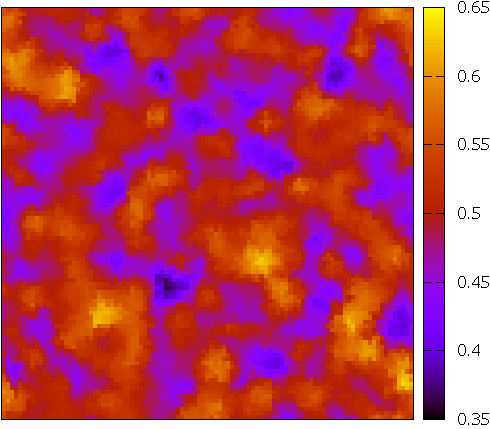
\includegraphics[scale=1]{pictures/voter_mod-crop.pdf}
\caption{Modified voter model stationary state on a 2D lattice. Opinions are in the interval $[0,1]$}
\label{fig:voter.mod}
\end{figure}

One of the first interesting things that is possible to see, is that the modified voter model, the one in which the opinions of people fill an entire continuum interval, has a stationary state, that looks like the one in Figure \ref{fig:voter.mod}. However, it is also possible to notice that, even if the initial distribution was a uniform distribution over the interval $[0,1]$, the distribution is changed at the stationary state, and it is neither uniform nor over the the same interval.
If in this situation the candidate are able to sample the opinions of the population, they both change their policy to be the median of the population distribution.

As soon as we introduce the possibility for the candidates to influence the opinions of people, the easy guess is that the opinions of people and the ones of the candidates converge towards the same stable value, and that is exactly what happens. Of course there will be fluctuations, and people will choose to vote the candidate which is closer to them. What is possible to see, is that in the end fluctuations decide the outcome of elections, and that both candidates have the same probability to win. Thus, even if \emph{everybody agrees with everybody}, fluctuations make the outcome of the electoral competition very unpredictable.

A similar thing happens when considering a more complex situation, when for instance there are three different candidates.
A stationary states is reached in which everybody basically agrees with everybody, with very small fluctuations that govern the dynamics of the system. Since the opinions are distributed with a very narrow symmetric distribution centred on the median, the candidate whose policy is in the middle of the other two candidates always get a very negligible number of votes, while the other two candidates are equally probable to be elected. But looking at the stationary state for some time steps allows to see the situation is always changing, with all of the candidates passing about a third of the time in the middle of the other two. This means that, even with simulations, it is impossible to predict the outcome of the elections in these conditions.

Going back to the case of only two candidates, the model also shows that if one of the two candidates possess information about the opinion distribution, that candidate is going to wind the election with certainty. That is because the other candidate does not know where the median is and thus cannot shift her policy.

Finally, it is interesting to see the how the probability of winning varies with the amount of information available to the candidates. To study this, the amount of information available to one of the candidates is kept constant, while the one available to the other spans a certain range. In particular while candidate one always gets information about $1\%$ of population, candidate one gets information for a value in $[0.2\%,5\%]$ in steps of $0.2$. It is possible to see that there is in fact a dependence of the 
probability of being elected on the amount of information that the candidates possesses, but it is very slight.
The candidates initial policy are $p_1=0$ and $p_2=1$, while the population have opinions uniformly distributed in $[0,1]$.

\section*{Conclusions}

The modifications introduced are very simple if taken one at a time, but together they significantly alter in a complex way both the Voter and Hotelling model.
It is evident that, whenever one wants to take a general model and make it a little bit more realistic, it is necessary to make assumptions and most of the time they are completely arbitrary and are chosen only because they are reasonable. Thus, this is one of the biggest difficulties in modelling and simulating social complex systems.

What is possible to see from the results is that the ideas and opinions of people change in a very complex way due to may different factors, and all of these factors influence each other in a way that is very difficult, if not impossible, to predict.
By refining tools like this, one could think that being in possess even of a little amount of information about the opinions of people could make a great difference in the strategies of candidates for political elections or in the strategies of private companies or individuals who would benefit from one outcome rather than one other. Moreover, just knowing this information is not enough to win the elections, but a lot of effort (and money) is being put by campaign managers on improving their candidate's presence online on the social media (like Twitter just to name one) because this is seen as a very important and determinant factor in winning the elections.
There are companies that are starting using Twitter and online scraping for polling instead of classical surveys since this is seen as a cheaper method, even if less accurate, to get feedback of gathering preliminary informations before deciding a certain policy.
Thus simulating this kind of systems can be helpful to get even just a qualitative idea of the consequences of certain actions, choices or strategies.

This trend is increasing very fast, and this poses doubt and questions on how data are used, about the ethic of data usage, and about the fact that if people are obtaining always better tools to influence the opinions and decisions of other people, maybe it will necessary to revise how this whole decision process works.
Luckily, social systems are very good in adapting to these novelties, and probably just taking conscience of the existence of these tools and how they work would be enough to quench the apparent threat that they pose. 

\end{document}

